\subsection{Search Queries for Literature Search in the Scientific Databases}
\label{appendix:search_queries}

\begin{table}[H]
    \centering
    \caption[Database Specific Search Queries Based on the Same Keywords]{Database search queries.}
    \label{table:database_search_queries}
    \small
    \begin{adjustbox}{width=1\textwidth,center}
    \begin{tabular}{lp{0.85\textwidth}}
        \toprule
        \textbf{Database} & \textbf{Search query} \\
        \midrule
        \text{Web of Science} & \texttt{TS=("AI" OR "ML" OR "Artificial intelligence" OR "Machine learning" OR "deep learning" OR "reinforcement learning" OR "supervised learning") AND TS=("probabilistic" OR "uncertainty quantification" OR "prediction intervals" OR "confidence intervals" OR "distributional forecast" OR "bayesian" OR "Gaussian process" OR "Undirected graphical models" OR "Markov Networks" OR "Markov random fields" OR "Probabilistic Graphical Models" OR "Variational inference" OR "Monte Carlo inference" OR "Hidden Markov models" OR "Gaussian mixture models" OR "Variational Autoencoders" OR "Dirichlet Process" OR "Stochastic Variational Inference") AND TS=("Forecast" OR "forecasting" OR "predict" OR "prediction" OR "estimate" OR "estimation") AND TS=("cryptocurrency" AND "bitcoin" OR "foreign exchange" OR "equity market*" OR "stock price*" OR "stock market*" OR "commodities" OR "value-at-risk" OR "value at risk" OR "CVaR" OR "expected shortfall" OR "forex" OR "financial time series" OR "stock trend*" OR "implied volatility" OR "realized volatility" OR ("volatility" AND "financ*"))} \\
        \addlinespace
        \hdashline[0.2pt/3pt]
        \addlinespace
        \text{Scopus} & \texttt{(TITLE-ABS-KEY("AI" OR "ML" OR "Artificial intelligence" OR "Machine learning" OR "deep learning" OR "reinforcement learning" OR "supervised learning") AND TITLE-ABS-KEY("probabilistic" OR "bayesian" OR "Gaussian process" OR "uncertainty quantification" OR "prediction intervals" OR "confidence intervals" OR "distributional forecast" OR "Undirected graphical models" OR "Markov Networks" OR "Markov random fields" OR "Probabilistic Graphical Models" OR "Variational inference" OR "Monte Carlo inference" OR "Hidden Markov models" OR "Gaussian mixture models" OR "Variational Autoencoders" OR "Dirichlet Process" OR "Stochastic Variational Inference") AND TITLE-ABS-KEY("Forecast" OR "forecasting" OR "predict" OR "prediction" OR "estimate" OR "estimation") AND TITLE-ABS-KEY("cryptocurrency" OR "bitcoin" OR "foreign exchange" OR "equity market*" OR "stock price*" OR "stock market*" OR "commodities" OR "value-at-risk" OR "value at risk" OR "CVaR" OR "expected shortfall" OR "forex" OR "financial time series" OR "stock trend*" OR "implied volatility" OR "realized volatility" OR ("volatility" AND "financ*"))) AND (LIMIT-TO(DOCTYPE, "ar") OR LIMIT-TO(DOCTYPE, "re")) AND (LIMIT-TO(LANGUAGE, "English"))} \\
        \addlinespace
        \hdashline[0.2pt/3pt]
        \addlinespace
        \text{ProQuest} & \texttt{SUMMARY,IF,TITLE(("AI" OR "ML" OR "Artificial intelligence" OR "Machine learning" OR "deep learning" OR "reinforcement learning" OR "supervised learning") AND ("probabilistic" OR "bayesian" OR "Gaussian process" OR "uncertainty quantification" OR "prediction intervals" OR "confidence intervals" OR "distributional forecast" OR "Undirected graphical models" OR "Markov Networks" OR "Markov random fields" OR "Probabilistic Graphical Models" OR "Variational inference" OR "Monte Carlo inference" OR "Hidden Markov models" OR "Gaussian mixture models" OR "Variational Autoencoders" OR "Dirichlet Process" OR "Stochastic Variational Inference") AND ("Forecast" OR "forecasting" OR "predict" OR "prediction" OR "estimate" OR "estimation") AND ("cryptocurrency" OR "bitcoin" OR "foreign exchange" OR "equity market*" OR "stock price*" OR "stock market*" OR "commodities" OR "value-at-risk" OR "value at risk" OR "CVaR" OR "expected shortfall" OR "forex" OR "financial time series" OR "stock trend*" OR "implied volatility" OR "realized volatility" OR ("volatility" AND "financ*"))) AND stype.exact("Scholarly Journals" OR "Dissertations \& Theses") AND la.exact("ENG")} \\
        \addlinespace
        \hdashline[0.2pt/3pt]
        \addlinespace
        \text{IEEE Xplore} & \texttt{(("AI" OR "ML" OR "Artificial intelligence" OR "Machine learning" OR "deep learning" OR "reinforcement learning" OR "supervised learning") AND ("probabilistic" OR "uncertainty quantification" OR "prediction intervals" OR "confidence intervals" OR "distributional forecast" OR "bayesian" OR "Gaussian process" OR "Undirected graphical models" OR "Markov Networks" OR "Markov random fields" OR "Probabilistic Graphical Models" OR "Variational inference" OR "Monte Carlo inference" OR "Hidden Markov models" OR "Gaussian mixture models" OR "Variational Autoencoders" OR "Dirichlet Process" OR "Stochastic Variational Inference") AND ("Forecast" OR "forecasting" OR "predict" OR "prediction" OR "estimate" OR "estimation") AND ("cryptocurrency" OR "bitcoin" OR "foreign exchange" OR "equity market*" OR "stock price*" OR "stock market*" OR "commodities" OR "value-at-risk" OR "value at risk" OR "CVaR" OR "expected shortfall" OR "forex" OR "financial time series" OR "stock trend*" OR "implied volatility" OR "realized volatility" OR ("volatility" AND "financ*")))} \\
        \bottomrule
    \end{tabular}
    \end{adjustbox}
\end{table}

\subsection{Screening Process in Detail}
\label{appendix:screening_process_with_ai}

[INTRO] + [LINK TO REPO] https://github.com/tjespe/literature-review

\textbf{Screening Phase 1: Initial Screening}

\begin{figure}[H]
     \centering
     \begin{subfigure}[b]{0.49\textwidth}
         \centering
         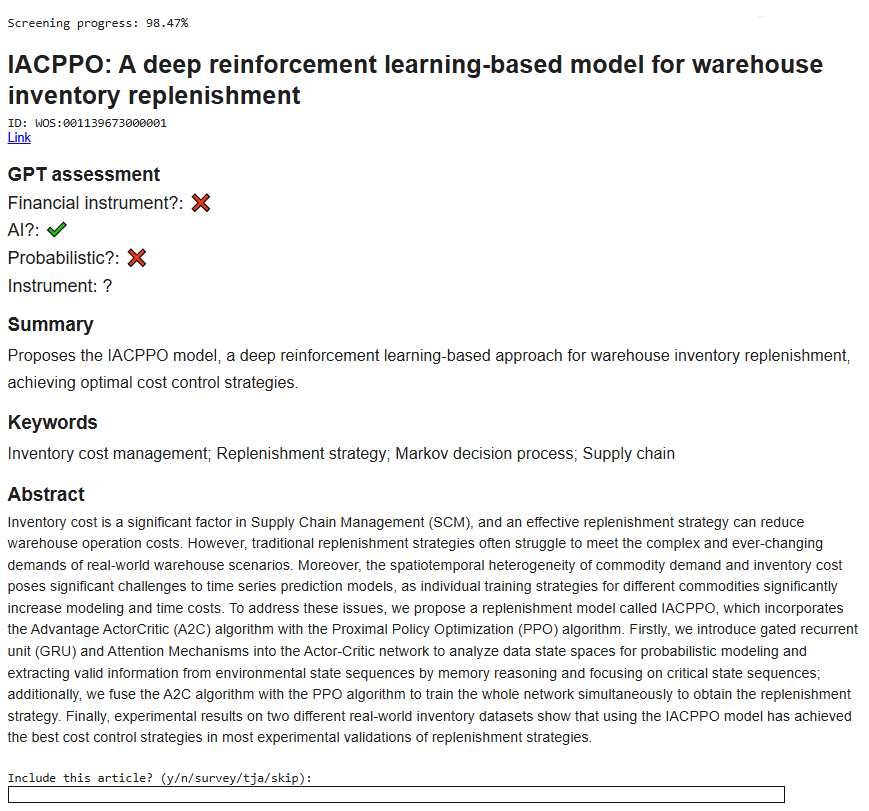
\includegraphics[width=\textwidth]{Images/screening_a.png}
         \caption{Example of article excluded in Screening Phase 1}
         \label{fig:screening_phase_1_rejected}
     \end{subfigure}
     \hfill
     \begin{subfigure}[b]{0.49\textwidth}
         \centering
         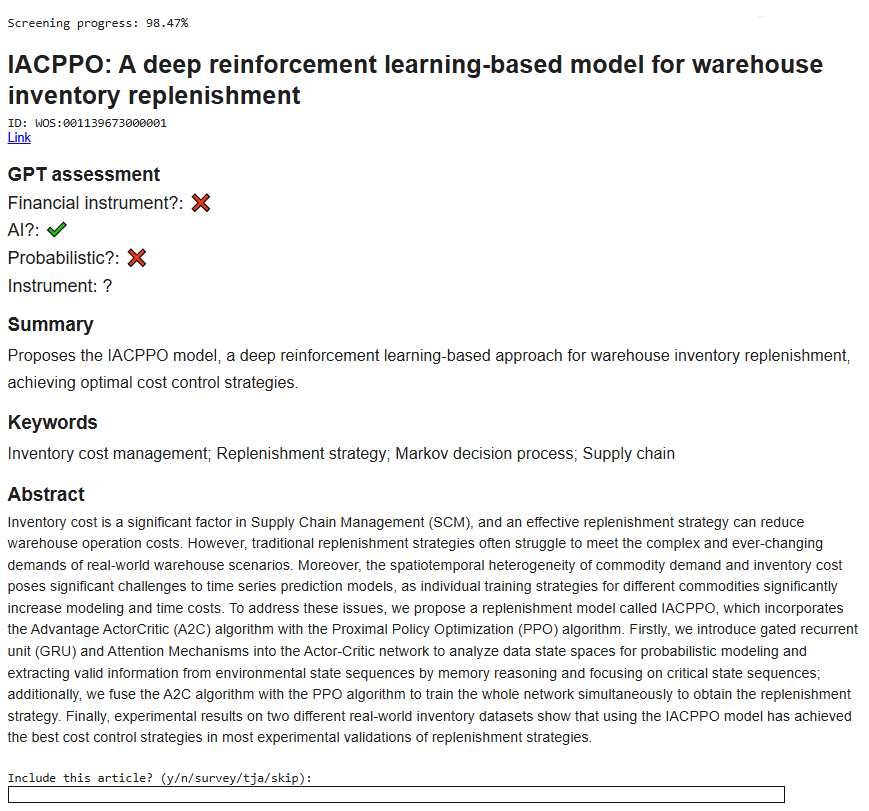
\includegraphics[width=\textwidth]{Images/screening_a.png}
         \caption{Example of article included in Screening Phase 1}
         \label{fig:screening_phase_1_included}
     \end{subfigure}
      \caption{Example of presented papers to the reviewer in Screening Phase 1. Researchers are prompted with a choice to include or exclude the paper based on the title, summary, keywords, and abstract. A link to the PDF of the paper is also included to perform a more thorough scan of the article in cases of doubt together with an AI assessment base on a large language model (“o1-mini” from OpenAI).}
    \label{fig:scrining_procces_phase_1}
\end{figure}


\textbf{Screening Phase 2: Full-text screening, Data extraction and Analysis}
\begin{figure}[H]
    \centering
    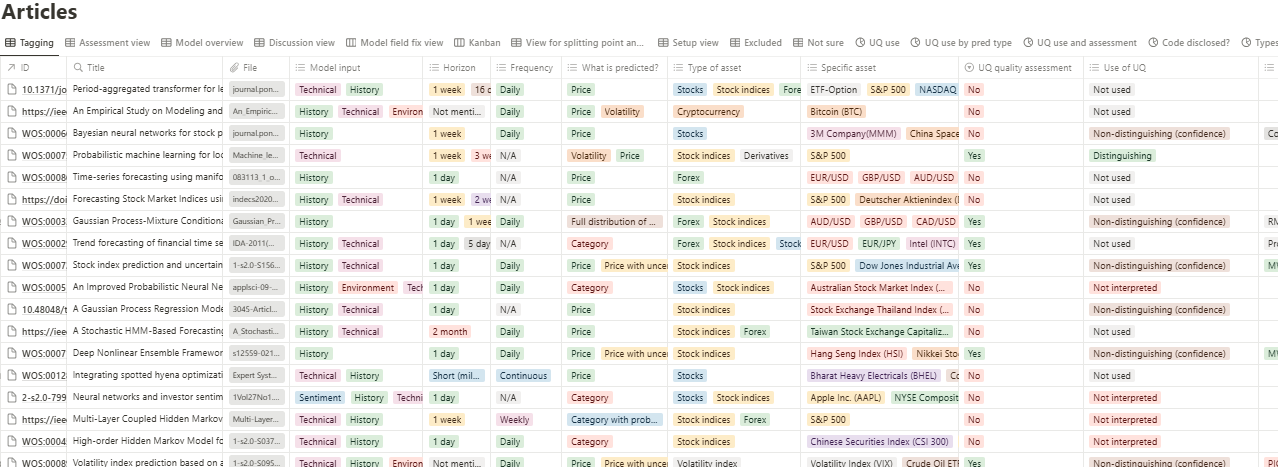
\includegraphics[width=1\linewidth]{Images/screening_process_tagging.png}
    \caption{Snapshot of dynamic table for tagging and data extraction of the papers during the full-text screening. The datatable wwas then loden into  }
    \label{fig:enter-label}
\end{figure}



\subsection{Journal Category Mapping}
\label{appendix:journal_category_mapping}

\begin{table}[H]
    \centering
    \caption[Journal Categories Mapping]{List of Journal Categories and Journals.}
    \label{table:journal_categories}
    \small
    \begin{adjustbox}{width=1\textwidth,center}
    \begin{tabular}{p{0.20\textwidth} p{0.80\textwidth}}
        \toprule
        \textbf{Category} & \textbf{Journals} \\
        \midrule
        Engineering and Technical & IEEE Access, IEEE Transactions on Computational Social Systems, Mobile Information Systems, The Institute of Electrical and Electronics Engineers, Inc. (IEEE) Conference Proceedings, IEEE Transactions on Industrial Informatics, Sensors, CMC-Computers Materials \& Continua, Journal of Theoretical and Applied Information Technology, Frontiers in Energy Research \\
        \addlinespace
        \hdashline[0.2pt/3pt]
        \addlinespace
        Computer Science and Artificial Intelligence & Expert Systems with Applications, Applied Soft Computing, IEEE Transactions on Artificial Intelligence, International Journal of Data Science and Analytics, IEEE Transactions on Neural Networks and Learning Systems, Machine Learning with Applications, Engineering Applications of Artificial Intelligence, Neural Networks, Expert Systems, Knowledge-Based Systems, IEEE Transactions on Systems, Man, and Cybernetics, Part B (Cybernetics), Cognitive Computation, Intelligent Data Analysis, IEEE Transactions on Pattern Analysis and Machine Intelligence, AI Communications, PeerJ Computer Science, Neural Computing and Applications, Neurocomputing, International Journal of Artificial Intelligence, Knowledge-Based Systems \\
        \addlinespace
        \hdashline[0.2pt/3pt]
        \addlinespace
        Multidisciplinary and General Science & PLoS ONE, Technological Forecasting and Social Change, Trends in Sciences, Sustainability, Applied Sciences-Basel, Stat, Interdisciplinary Description of Complex Systems, Resources Policy \\
        \addlinespace
        \hdashline[0.2pt/3pt]
        \addlinespace
        Economics, Finance, and Business & Quantitative Finance, SIAM Journal on Financial Mathematics, Journal of Risk Model Validation, Digital Finance, Computational Economics, Research in International Business and Finance, Financial Analysts Journal, International Journal of Economics and Business Research, Revista Perspectiva Empresarial, Journal of Forecasting, Journal of Computational Finance \\
        \addlinespace
        \hdashline[0.2pt/3pt]
        \addlinespace
        Physics and Mathematics & Physica A-Statistical Mechanics and its Applications, Chaos, Journal of Physics: Conference Series, Communications in Applied Mathematics and Computational Science, Mathematics, Mathematics and Computers in Simulation, IAENG International Journal of Applied Mathematics, Journal of Statistical Computation and Simulation, Technometrics \\
        \bottomrule
    \end{tabular}
    \end{adjustbox}
\end{table}


\subsection{List of Abbreviations}
\label{appendix:list_of_abbrevations}
    

\begin{table}[H]
    \centering
    \caption[List of Abbreviations]{List of Abbreviations.}
    \label{table:abbreviations}
    \small
    \begin{subtable}[t]{0.49\textwidth}
        \centering
        \begin{tabular}{lp{0.63\textwidth}}
        \toprule
        \textbf{Abbreviation} & \textbf{Definition} \\
        \midrule
        ADAM & Adaptive Moment Estimation \\
        AE & Auto-Encoder \\
        AIS & Average Internal Score \\
        AI & Artificial Intelligence \\
        ANN & Artificial Neural Network \\
        ARIMA & AutoRegressive Integrated Moving Average \\
        AUROC & Area Under the ROC Curve \\
        BGLM & Bayesian Generalized Linear Model \\
        BIC & Bayesian Information Criterion \\
        BNN & Bayesian Neural Network \\
        B-SLR & Bibliometric Systematic Literature Review \\
        B-SVR & Bayesian Support Vector Regression \\
        BSTS & Bayesian Structural Time-Series \\
        B-TABL & Bayesian Temporal Augmented Bilinear Network \\
        cGAN & Conditional Generative Adversarial Networks \\
        CDF & Cumulative Distribution Functions \\
        CNN & Convolutional Neural Networks \\
        CoV & Coefficient of Variation \\
        CPS & Conformal Predictive System \\
        CRPS & Continuous Ranked Probability Score \\
        CVaR / ES & Conditional Value at Risk / Expected Shortfall \\
        DCNN & Deep Convolutional Neural Network \\
        DNN & Deep Neural Network \\
        DQ & Dynamic Quantile \\
        ECE & Expected Calibration Error \\
        ECD & Expected Calibration Distance \\
        EGARCH & Exponential GARCH \\
        ESVM & Echo State Volatility Model \\
        EWSVM & Enhanced Weighted Support Vector Machine \\
        FINAW & Forecasting Interval Normalized Average Width \\
        FF-ANN & Feed-Forward Artificial Neural Network \\
        FFNN & Feed-Forward Neural Network \\
        GAN & Generative Adversarial Network \\
        GA & Genetic Algorithms \\
        GBHM & Bayesian General Heteroskedasticity Model \\
        GP & Gaussian Process \\
        GPMCH & Gaussian Process Mixture Conditional Heteroscedasticity \\
        GPR & Gaussian Processes Regression \\
        GARCH & Generalized Autoregressive Conditional Heteroskedasticity \\
        GRU & Gated Recurrent Units \\
        HMM & Hidden Markov Model \\
        
        
        \bottomrule
        \end{tabular}
    \end{subtable}
    \hfill
    \begin{subtable}[t]{0.49\textwidth}
        \centering
        \begin{tabular}{lp{0.63\textwidth}}
        \toprule
        \textbf{Abbreviation} & \textbf{Definition} \\
        \midrule
        IMF & Intrinsic Mode Functions \\
        ITM & In-The-Money \\
        IVOL & Implied Volatility \\
        LOB & Limit Order Books \\
        LOO-CCPS & Leave-One-Out Cross-Conformal Predictive System \\
        LSTM & Long Short-Term Memory \\
        MAE & Mean Absolute Error \\
        MC & Mean Coverage \\
        MCUB & Multi-Class Undersampling-Based Bagging \\
        MCHMM & Multi-Layer Coupled Hidden Markov Model \\
        MCMC & Markov Chain Monte Carlo \\
        MLP & Multilayer Perceptron \\
        ML & Machine Learning \\
        MNF & Minimum Norm Filter \\
        MSEV & Mean Squared Error of Variance \\
        MWP & Mean Width Percentage \\
        NLL & Negative Log-Likelihood \\
        NSE & Nash–Sutcliffe Model Efficiency Coefficient \\
        OTM & Out-Of-The-Money \\
        PICP & Prediction Interval Coverage Probability \\
        PINAW & Prediction Interval Normalized Average Width \\
        PredACGAN & Predictive Auxiliary Classifier GAN \\
        PDF & Probability Density Functions \\
        PNN & Probabilistic Neural Network \\
        QL & Quantile Loss \\
        QR & Quantile Regression \\
        RDL & Recurrent Dictionary Learning \\
        RELM & Regularized Extreme Learning Machine \\
        RMSCE & Root Mean Squared Calibration Error \\
        RT & Reparametrization Trick \\
        SAVING & Sentiment-Aware Volatility Forecasting \\
        SHOA & Spotted Hyena Optimization Algorithm \\
        SLR & Systematic Literature Review \\
        SSA & Singular Spectrum Analysis \\
        SSE & Sum of Squared Errors \\
        SVM & Support Vector Machines \\
        SVR & Support Vector Regression \\
        TARCH & Threshold GARCH \\
        TCN & Temporal Convolutional Network \\
        TVaR & Tail Value at Risk \\
        UCRP & Uniform Constant Rebalanced Portfolio \\
        VaR & Value at Risk \\
        VAE & Variational Autoencoder \\
        VDM & Variational Mode Decomposition \\
        VOGN & Variational Online Gauss-Newton \\
        XAI & Explainable AI \\
        \bottomrule
        \end{tabular}
    \end{subtable}
\end{table}



\subsection{Journals per Category}






\subsection{Descriptive Table of all Papers in Sample}
\label{appendix:descriptive_table_of_all_articles}

\scriptsize % Adjust font size for the table
\setlength\LTcapwidth{\textheight} % Ensure the caption matches the rotated height

% Rotate the table while allowing it to span multiple pages
\begin{landscape}
\begin{longtable}{p{0.07\textheight} p{0.07\textheight} p{0.16\textheight} p{0.07\textheight} p{0.07\textheight} p{0.07\textheight} p{0.14\textheight} p{0.07\textheight} p{0.07\textheight} p{0.07\textheight} p{0.07\textheight} p{0.1\textheight} p{0.04\textheight}}
        \caption[Descriptive table of all papers in sample]{Summary of Paper Information}
        \label{table:paper_info_summary} \\
        \toprule
        \textbf{Reference} & \textbf{Asset category} & \textbf{Asset} & \textbf{Input} & \textbf{Horizon} & \textbf{Predicted} & \textbf{Prob. AI Model} & \textbf{Composed with ML Model} & \textbf{Composed with Trad. model} & \textbf{Use of UQ} & \textbf{UQ Quality Assessment} & \textbf{Assessment Criteria UQ} & \textbf{Code} \\
        \midrule
        \endfirsthead

        \toprule
        \textbf{Reference} & \textbf{Asset category} & \textbf{Asset} & \textbf{Input} & \textbf{Horizon} & \textbf{Predicted} & \textbf{Prob. AI Model} & \textbf{Composed with ML Model} & \textbf{Composed with Trad. model} & \textbf{Use of UQ} & \textbf{UQ Quality Assessment} & \textbf{Assessment Criteria UQ} & \textbf{Code} \\
        \midrule
        \endhead

        \midrule
        \multicolumn{13}{r}{\textit{Continued on next page}} \\
        \midrule
        \endfoot

        \bottomrule
        \endlastfoot

         \textcite{Almeida2024RiskForecasting} & Cryptocurrency & Ethereum portfolio & History, Technical & 1 day & Distributional Forecast, Financial Risk Measure & DeepAR (based on autoregressive RNN) & N/A & N/A & Financial interpretation (e.g. VaR) & Yes & Continuous Ranked Probability Score (CRPS), Elicitability score for VaR & No \\
        \addlinespace
        \hdashline[0.2pt/3pt]
        \addlinespace
        
        \textcite{Chandrasekara2019pnn} & Stock indices, Stocks & Australian Stock Market Index (AORD), S\&P 500, Sri Lankan Stock Market Index (ASPI) & Environment, History, Technical & 1 day & Category & Probabilistic Neural Network (PNN) & multi-class undersampling-based bagging (MCUB) & N/A & Not interpreted & No & N/A & No \\
        \addlinespace
        \hdashline[0.2pt/3pt]
        \addlinespace
        
        \textcite{Daniali2021} & Volatility index & Volatility Index (VIX) & History, Technical & 1 day & Price, Volatility & Deep Convolutional Neural Network (DCNN) & N/A & Conditional Variance model & Not used & No & N/A & No \\
        \addlinespace
        \hdashline[0.2pt/3pt]
        \addlinespace
        
        \textcite{DeSpiegeleer2018gpr} & Derivatives & S\&P 500 American Options, S\&P 500 European Options & Environment, History, Technical & Not mentioned & Distributional Forecast & Gaussian Process Regression (GPR) & N/A & N/A & Not interpreted & No & N/A & No \\
        \addlinespace
        \hdashline[0.2pt/3pt]
        \addlinespace
        
        \textcite{Dixon2022Industrial} & Stocks & International Business Machines (IBM) & History & 1 day, 5 days & Distributional Forecast & Bayesian exponential smoothed RNNs (Bayes ES-RNN) (BNN) & N/A & N/A & Non-distinguishing (confidence) & Yes & Coverage probabillty & No \\
        \addlinespace
        \hdashline[0.2pt/3pt]
        \addlinespace
        
        \textcite{Fatouros2023DeepVaR} & Portfolio & AUD/USD, EUR/USD, GBP/USD, USD/JPY & History, Technical & 1 day & Distributional Forecast, Financial Risk Measure & DeepAR (based on autoregressive RNN) & N/A & N/A & Financial interpretation (e.g. VaR) & Yes & Christoffersen’s Test, Conditional Coverage Test, Dynamic Quantile (DQ), Firm Loss, Quadratic Loss (QL), Smooth Loss, Unconditional Coverage Test & Yes \\
        \addlinespace
        \hdashline[0.2pt/3pt]
        \addlinespace
        
        \textcite{Golnari2024Cryptocurrency} & Cryptocurrency & Bitcoin (BTC), Cardano (ADA), Ethereum (ETH), Litecoin (LTC), Polkadot (DOT), Stellar (XLM), Tron (TRX) & History, Technical & 5 minutes & Distributional Forecast & Probabilistic Gated Recurrent Units (P-GRU) & N/A & N/A & Non-distinguishing (confidence) & No & N/A & Yes \\
        \addlinespace
        \hdashline[0.2pt/3pt]
        \addlinespace
        
        \textcite{Grudniewicz2023Application} & Stock indices & Budapest Stock Exhange Index (BUX), Bulgaria Stock Exchange Index (SOFIX), Deutscher Aktienindex (DAX), OMX Riga Index (OMXR), OMX Tallin Index (OMXT), OMX Vilnius Index (OMXV), Prague Stock Exchange Index (PX), S\&P 500, Warsaw Stock Exchange Index (WIG20) & History, Technical & 20 days & Category & Bayesian Generalized Linear Model (BGLM), Naïve Bayes (NB) & N/A & N/A & Not used & No & N/A & No \\
        \addlinespace
        \hdashline[0.2pt/3pt]
        \addlinespace
        
        \textcite{Hassan2024Bitcoin} & Cryptocurrency & Bitcoin (BTC) & History & 1 day & Distributional Forecast & Bayesian LSTM with Monte Carlo Drouput & N/A & N/A & Epistemic (Model) & No & N/A & No \\
        \addlinespace
        \hdashline[0.2pt/3pt]
        \addlinespace
        
        \textcite{Hocht2024gpr} & Capped volatility swaps & Apple Inc. (AAPL), JPMorgan Chase \& Co (JPM), S\&P 500 & Environment, History, Technical & Flexible & Volatility & Gaussian Process Regression (GPR) & N/A & N/A & Not used & No & N/A & No \\
        \addlinespace
        \hdashline[0.2pt/3pt]
        \addlinespace
        
        \textcite{Horenko2020} & Stock indices & Dow Jones Industrial Average (DJI), EURO STOXX 50 (STOXX), FTSE 100, Hang Seng Index (HSI), Nikkei Stock Average (NI225), S\&P 500, Swiss Market Index (SMI) & History, Technical & 1 day & Distributional Forecast, Financial Risk Measure & TV-Entropy & N/A & N/A & Aleatoric (Volatility), Financial interpretation (e.g. VaR) & Yes & Bayesian Information Criteria (BIC), Coverage probabillty, Kupiec’s test, negative log-likelihood (NLL) & Yes \\
        \addlinespace
        \hdashline[0.2pt/3pt]
        \addlinespace
        
        \textcite{Lahmiri2024pnn} & Stock indices, Stocks & Apple Inc. (AAPL), Cisco Systems (CSCO), General Electric (GE), NYSE Composite & History, Sentiment, Technical & 1 day & Category & Probabilistic Neural Network (PNN) & N/A & N/A & Not interpreted & No & N/A & No \\
        \addlinespace
        \hdashline[0.2pt/3pt]
        \addlinespace
        
        \textcite{Law2017Practical} & Bonds, Commodities, Credit Default Swap (CDS) Spreads, Stock indices & CME Gold Front Month Futures, FTSE 100, IBM-CDS 5YR, ICE BRENT Crude Oil Front Month Futures, S\&P 500, UK Gilt 10YR Bond Yield, US Treasury 10YR Bond Yield, WMT-CDS 5YR & History & 1 day & Distributional Forecast & Bayesian Support Vector Regression (B-SVR) & N/A & N/A & Non-distinguishing (confidence) & Yes & Correlation between uncertainty and prediction error & No \\
        \addlinespace
        \hdashline[0.2pt/3pt]
        \addlinespace
        
        \textcite{Li2024DeepAR} & Stocks & Chinese company stocks & History & Flexible & Distributional Forecast & DeepAR with attention (DeepARA) & N/A & N/A & Non-distinguishing (confidence) & Yes & Entropy of probability distribution & No \\
        \addlinespace
        \hdashline[0.2pt/3pt]
        \addlinespace
        
        \textcite{Li2024gpr} & Portfolio & MSCI World Index (MSCI), New York Stock Exchange (NYSE) stock portfolio, S\&P 500, Toronto Stock Exchange (TSE) stock portfolio & History, Technical & 1 day & Distributional Forecast & Graph-Aware Gaussian Process (G4P) & N/A & N/A & Non-distinguishing (confidence) & Yes & Portfolio construction and evaluation & Yes \\
        \addlinespace
        \hdashline[0.2pt/3pt]
        \addlinespace
        
        \textcite{Malagrino2018Forecasting} & Stock indices & Bombay Stock Exchange (BSE 30 SENSEX), Cotation Assistée en Continu (CAC 40), Deutscher Aktienindex (DAX), Dow Jones Industrial Average (DJI), FTSE 100, Hang Seng Index (HSI), Merval (MERV), NASDAQ Composite, NYSE Composite, Nikkei Stock Average (NI225), Shanghai Composite (SSE), Stockholm General (OMXS 30) & Environment, History, Technical & 1 day, 2 days, 20 days & Category & Bayesian Neural Network (BNN) & N/A & N/A & Not interpreted & No & N/A & No \\
        \addlinespace
        \hdashline[0.2pt/3pt]
        \addlinespace
        
        \textcite{Maniatopoulos2022pnn} & Stocks & US Dow Jones Stocks & Environment, History, Technical & 10 days, 15 days, 20 days, 5 days & Category & probabilistic feed-foward neural network (P FF-ANN) & N/A & N/A & Not used & No & N/A & No \\
        \addlinespace
        \hdashline[0.2pt/3pt]
        \addlinespace
        
        \textcite{Min2023BlackLitterman} & Portfolio, Stocks & S\&P 500 stock portfolio & History & 50 months & Distributional Forecast & Gaussian Process Regression (GPR) & N/A & Black-Litterman & Non-distinguishing (confidence) & Yes & Portfolio construction and evaluation & No \\
        \addlinespace
        \hdashline[0.2pt/3pt]
        \addlinespace
        
        \textcite{Papaioannou2022gpr} & Forex & AUD/USD, CAD/USD, CHF/USD, DKK/USD, EUR/USD, GBP/USD, JPY/USD, NOK/USD, NZD/USD, SEK/USD & History & 1 day & Price & Gaussian Process Regression (GPR) & N/A & N/A & Not used & No & N/A & No \\
        \addlinespace
        \hdashline[0.2pt/3pt]
        \addlinespace
        
        \textcite{Park2014gpr} & Options & KOSPI 200 Index options & Technical & Flexible & Price & Gaussian Process Regression (GPR) & N/A & N/A & Not used & No & N/A & No \\
        \addlinespace
        \hdashline[0.2pt/3pt]
        \addlinespace
        
        \textcite{Park2024UncertaintyAware} & Portfolio, Stocks & KOSPI stocks, NASDAQ stocks, NYSE stocks & History, Technical & Short (milliseconds) & Distributional Forecast & risk-sensitive multiagent network (RSMAN) & N/A & N/A & Distinguishing & Yes & Portfolio construction and evaluation & No \\
        \addlinespace
        \hdashline[0.2pt/3pt]
        \addlinespace
        
        \textcite{Parker2021BayesianHeteroskedastic} & Stock indices & Dow Jones Industrial Average (DJI) & Environment, History, Technical & Not mentioned & Volatility & Echo State Volatility Model (ESVM) & N/A & N/A & Distinguishing & Yes & Coverage probabillty, MSEV & No \\
        \addlinespace
        \hdashline[0.2pt/3pt]
        \addlinespace
        
        \textcite{Platanios2014gpr} & Forex, Stock indices & AUD/USD, CAD/USD, CHF/USD, Canadian TSX Composite (TSX), Cotation Assistée en Continu (CAC 40), DEM/USD, DKK/USD, Deutscher Aktienindex (DAX), FRF/USD, FTSE 100, GBP/USD, JPY/USD, Nikkei Stock Average (NI225), S\&P 500 & History & 1 day, 1 week, 30 days & Distributional Forecast, Volatility & nonparametric Bayesian mixture of Gaussian process regression models (GPMCH) & N/A & N/A & Non-distinguishing (confidence) & Yes & RMSE (against squared returns) & No \\
        \addlinespace
        \hdashline[0.2pt/3pt]
        \addlinespace
        
        \textcite{Raúl_PlazaCasado_PradoRomán_2021} & Stock indices & IBerian Index (IBEX) & History, Sentiment & 1 day & Category & Bayesian Network (BN) & N/A & N/A & Non-distinguishing (confidence) & Yes & Success rate & No \\
        \addlinespace
        \hdashline[0.2pt/3pt]
        \addlinespace
        
        \textcite{Risk2018gpr} & Portfolio & N/A & Environment, History & 1 year & Distributional Forecast, Financial Risk Measure & Gaussian Process Regression (GPR) & N/A & N/A & Distinguishing, Financial interpretation (e.g. VaR) & Yes & RMSE (against Harrell-Davis as ground truth) & No \\
        \addlinespace
        \hdashline[0.2pt/3pt]
        \addlinespace
        
        \textcite{Sharma2021} & Stocks & Chinese company stocks, India stocks, UK stocks, USA stocks & History & 1 day & Category, Distributional Forecast & Recurrent Dictionary Learing (RDL) & N/A & N/A & Non-distinguishing (confidence) & Yes & Log-loss & No \\
        \addlinespace
        \hdashline[0.2pt/3pt]
        \addlinespace
        
        \textcite{Suphawan2022gpr} & Stock indices & Stock Exchange Thailand Index (SET) & History, Technical & 1 day & Distributional Forecast & Gaussian Process Regression (GPR) & N/A & N/A & Non-distinguishing (confidence) & No & N/A & No \\
        \addlinespace
        \hdashline[0.2pt/3pt]
        \addlinespace
        
        \textcite{Thawornwong2004pnn} & Portfolio & S\&P 500 stock portfolio & Environment, Fundamental, History, Technical & 1 month & Category & Probabilistic Neural Network (PNN) & N/A & N/A & Not used & No & N/A & No \\
        \addlinespace
        \hdashline[0.2pt/3pt]
        \addlinespace
        
        \textcite{Tian2023} & Volatility index & 10-Year U.S. treasury note volatility index (TYVIX), Crude Oil ETF Volatility Index (COEVI), Volatility Index (VIX) & Environment, History, Technical & Not mentioned & Distributional Forecast, Volatility & Fitting error analysis & Clockwork Recurrent Neural Network (CWRNN), Cuckoo-Search-enhanced Multi-Objective Grey Wolf Optimizer (MOGWOCS) & N/A & Non-distinguishing (confidence) & Yes & PICP (Prediction interval coverage probability), Prediction Interval Normalized Average Width (PINAW), Winkler Score, coverage widthbased criterion (CWC) & No \\
        \addlinespace
        \hdashline[0.2pt/3pt]
        \addlinespace
        
        \textcite{Wang2021gprensemble} & Stock indices & Hang Seng Index (HSI), Nikkei Stock Average (NI225) & History & 1 day & Distributional Forecast & Gaussian Process Regression (GPR) & Enhanced Weighted Support Vector Machine (EWSVM), Recurrent Neural Network (RNN) & Singular Spectrum Analysis (SSA) & Non-distinguishing (confidence) & Yes & Coverage probabillty, MWP (Mean width percentage), Mean width divided by coverage probability & No \\
        \addlinespace
        \hdashline[0.2pt/3pt]
        \addlinespace
        
        \textcite{Wang2021gpr} & Stock indices & Dow Jones Industrial Average (DJI), NASDAQ Composite, S\&P 500 & History, Technical & 1 day & Distributional Forecast & Gaussian Process Regression (GPR) & Auto-Encoder (AE), Long Short Term Memory Neural Network (LSTM), Recurrent Neural Network (RNN), Variational Mode Decomposition (VMD) & N/A & Non-distinguishing (confidence) & Yes & MC (Mean coverage), MWP (Mean width percentage), PICP (Prediction interval coverage probability) & No \\
        \addlinespace
        \hdashline[0.2pt/3pt]
        \addlinespace
        
        \textcite{Wang2024GoldForecasting} & Commodities & Gold price & Environment, History, Sentiment & Not mentioned & Confidence Interval & Quantile Regression (QR), Quantile Regression Bi-Directional Long Short-Term Memory (QRBiLSTM) & N/A & N/A & Aleatoric (Volatility) & Yes & PICP (Prediction interval coverage probability), Prediction Interval Normalized Average Width (PINAW), Quantile loss (QL), Semi-interval metric, average interval score (AIS) & No \\
        \addlinespace
        \hdashline[0.2pt/3pt]
        \addlinespace
        
        \textcite{Zhang2016} & Stocks & NASDAQ stocks, Second-board Market of Shenzhen Stock Exchange (SZSE) stocks & History, Technical & Flexible & Category & Probabilistic Support Vector Machine (PSVM) & AdaBoost, Genetic Algorithm (GA) & N/A & Not interpreted & No & N/A & No \\
        \addlinespace
        \hdashline[0.2pt/3pt]
        \addlinespace
        
        \textcite{Zmuk2020gpr} & Stock indices & Deutscher Aktienindex (DAX), Dow Jones Industrial Average (DJI), NASDAQ Composite, Nikkei Stock Average (NI225), S\&P 500 & History, Technical & 1 month, 1 week, 2 weeks & Price & Gaussian Process Regression (GPR) & N/A & N/A & Not used & No & N/A & No \\
        \addlinespace
        \hdashline[0.2pt/3pt]
        \addlinespace
        
        \textcite{arian2022encoded} & Portfolio, Stocks & Frankfurt Stock Exchange (FSE) stock portfolio, London Stock Exchange (LSE) stock portfolio, S\&P 500 & History, Technical & 1 day & Distributional Forecast, Financial Risk Measure & Variational Auto-encoder (VAE) & N/A & N/A & Aleatoric (Volatility), Financial interpretation (e.g. VaR) & Yes & Christoffersen’s Test, Conditional Coverage Test, Independence Test, Kupiec’s test, Lopez' loss function, Unconditional Coverage Test & Yes \\
        \addlinespace
        \hdashline[0.2pt/3pt]
        \addlinespace
        
        \textcite{cao2019multi} & Forex, Stock indices & S\&P 500 & History, Technical & 1 week & Category & Multi-Layer Coupled Hidden Markov Model (MCHMM) & N/A & N/A & Not interpreted & No & N/A & No \\
        \addlinespace
        \hdashline[0.2pt/3pt]
        \addlinespace
        
        \textcite{caprioli2023quantifying} & Portfolio & Total Market Index Emerging Markets, Total Market Index Europe, Total Market Index Italy, Total Market Index US & History, Technical & 1 year & Financial Risk Measure & Variational Auto-encoder (VAE) & N/A & multi-factor Vasicek model & Financial interpretation (e.g. VaR) & Yes & the largest eigenvalue of the correlation matrix & No \\
        \addlinespace
        \hdashline[0.2pt/3pt]
        \addlinespace
        
        \textcite{chandra2021bayesian} & Stocks & 3M Company(MMM), China Spacesat Company Limited (600118.SS), Commonwealth Bank of Australia (CBA.AX), Daimler AG (DAI. DE) & History & 1 week & Distributional Forecast & Langevin-gradient Bayesian neural networks (BNN) with parallel tempering Markov Chain Monte Carlo (MCMC) & N/A & N/A & Non-distinguishing (confidence) & No & Confidence interval & Yes \\
        \addlinespace
        \hdashline[0.2pt/3pt]
        \addlinespace
        
        \textcite{choudhury2020enhancing} & Stocks & Adobe (ADBE), Amazon (AMZN), Apple Inc. (AAPL), Cerner Corporation (CERN), Costco (COST), Facebook (FB), Fastenal Company (FAST), Google (GOOG), Hasbro Inc (HAS), IDEXX Laboratories Inc. (IDXX), Intel (INTC) & History, Technical & 7-minutes & Price & Variational Auto-encoder (VAE) & Long Short Term Memory Neural Network (LSTM) & N/A & Not used & No & N/A & No \\
        \addlinespace
        \hdashline[0.2pt/3pt]
        \addlinespace
        
        \textcite{cocco2021predictions} & Cryptocurrency & Bitcoin (BTC), Ethereum (ETH) & Technical & 1 day, 1 month, 2 weeks & Distributional Forecast & BNN-SVR, Bayesian Neural Network (BNN) & N/A & N/A & Non-distinguishing (confidence) & No & N/A & No \\
        \addlinespace
        \hdashline[0.2pt/3pt]
        \addlinespace
        
        \textcite{govindasamy2014prediction} & Stocks & N/A & History, Technical & Not mentioned & Price & PECEP (Combo of Complex Event Processing [CEP] and Probabilistic Fuzzy Logic [PFL]) & N/A & N/A & Not used & No & N/A & No \\
        \addlinespace
        \hdashline[0.2pt/3pt]
        \addlinespace
        
        \textcite{hortua2024forecasting} & Derivative index & Volatility Index (VIX) & History & Not mentioned & Distributional Forecast & Bayesian Neural Network (BNN), WaveNet & Temporal Convolutional Network (TCN), Transformers & N/A & Distinguishing & Yes & Calibration diagrams, PICP (Prediction interval coverage probability), RMSCE, Scaling factor & No \\
        \addlinespace
        \hdashline[0.2pt/3pt]
        \addlinespace
        
        \textcite{jang2018empirical} & Cryptocurrency & Bitcoin (BTC) & Environment, History, Technical & Not mentioned & Price & Bayesian neural networks (BNNs) & N/A & N/A & Not used & No & N/A & No \\
        \addlinespace
        \hdashline[0.2pt/3pt]
        \addlinespace
        
        \textcite{jang2018generative} & Options & S\&P 100 American put options & Technical & 1 day, 1 week & Price & Generative Bayesian Neural Network (Gen-BNN) & N/A & N/A & Not used & No & N/A & No \\
        \addlinespace
        \hdashline[0.2pt/3pt]
        \addlinespace
        
        \textcite{kim2023portfolio} & Portfolio & NASDAQ 100 stocks portfolio, S\&P 500 stock portfolio & History, Technical & 1 month & Category & Predictive Auxiliary Classifier Generative Adversarial Networks (PredACGAN) & N/A & N/A & Non-distinguishing (confidence) & Yes & Entropy of probability distribution & Yes \\
        \addlinespace
        \hdashline[0.2pt/3pt]
        \addlinespace
        
        \textcite{lee2021estimation} & Stock indices & NASDAQ-100 Future Index & History, Technical & 1 week & Distributional Forecast & Conditional Generative Adversarial Network (CGAN) & N/A & N/A & Non-distinguishing (confidence) & Yes & Correlation between uncertainty and prediction error, Portfolio construction and evaluation & Yes \\
        \addlinespace
        \hdashline[0.2pt/3pt]
        \addlinespace
        
        \textcite{li2010stochastic} & Forex, Stock indices & Taiwan Stock Exchange Capitalization Weighted Stock Index (TAIEX) & History, Technical & 2 month & Price & Stochastic Hidden Markov Model (HMM) & N/A & N/A & Not used & No & N/A & No \\
        \addlinespace
        \hdashline[0.2pt/3pt]
        \addlinespace
        
        \textcite{li2020multivariate} & Commodities & Soybean Futures & Environment, Fundamental, History, Technical & Not mentioned & Price & Multimodal Variational Autoencoder (VAE) & Long Short Term Memory Neural Network (LSTM), Recurrent Neural Network (RNN) & N/A & Not used & No & N/A & No \\
        \addlinespace
        \hdashline[0.2pt/3pt]
        \addlinespace
        
        \textcite{magris2023bayesian} & Stocks & Nasdaq Nordic Helsinki Exchange Stocks & History, Technical & Short (milliseconds) & Category & Bayesian temporal attention augmented bilinear network (B-TABL) & N/A & N/A & Non-distinguishing (confidence) & Yes & Expected Calibration Distance (ECD), Expected Calibration Error (ECE) & No \\
        \addlinespace
        \hdashline[0.2pt/3pt]
        \addlinespace
        
        \textcite{park2011trend} & Forex, Stock indices, Stocks & Boeing (BA), EUR/JPY, EUR/USD, FTSE 100, Intel (INTC), S\&P 500, US-Treasury Bill 5YR, Walmart (WMT) & History, Technical & 1 day, 5 days & N/A & Continuous Hidden Markov Model (CHMM) & N/A & PIPs Detection Algorithm & Not used & Yes & Probabilistic Trend Prediction Precision (PTPP) & No \\
        \addlinespace
        \hdashline[0.2pt/3pt]
        \addlinespace
        
        \textcite{salama2024gan} & Stocks & Axis Bank (AXISBANK), Bharat Heavy Electricals (BHEL), Container Store Group (TSC), Maruti (MARUTI), Tata Steel (TATASTEEL), Wipro (WIPRO) & History, Technical & Short (milliseconds) & Price & Conditional Generative Adversarial Network (CGAN) & Spotted Hyena Optimization Algorithm (SHOA) & N/A & Not used & No & N/A & No \\
        \addlinespace
        \hdashline[0.2pt/3pt]
        \addlinespace
        
        \textcite{sher2023exploiting} & Stocks & Apple Inc. (AAPL), Broadcom Inc. (AVGO), Microsoft Corporation (MSFT), Nvidia Corporation (NVDA), Taiwan Semiconductor Manufacturing Company Limited (LSM) & History & Not mentioned & Category & Hidden Markov Model (HMM) & N/A & N/A & Not used & No & N/A & Yes \\
        \addlinespace
        \hdashline[0.2pt/3pt]
        \addlinespace
        
        \textcite{soleymani2022longterm} & Stocks & Advanced Micro Devices (AMD), Amazon (AMZN), Apple Inc. (AAPL), Google (GOOG), Microsoft Corporation (MSFT), Nvidia Corporation (NVDA), Pfizer (PFE), Shopify (SHOP), Walmart (WMT) & History, Technical & 10 days, 15 days, 20 days, 30 days, 5 days & Distributional Forecast & deep Bayesian neural networks (BNNs) & temporal generative adversarial neural networks (t-GAN) & N/A & Fed into other model & No & N/A & No \\
        \addlinespace
        \hdashline[0.2pt/3pt]
        \addlinespace
        
        \textcite{su2022hmm} & Stock indices & Hang Seng Index (HSI) & History, Technical & 1 month, 3 month, 6 month & Category, Price & Hidden Markov Model (HMM) & k-means clustering & N/A & Not used & No & N/A & No \\
        \addlinespace
        \hdashline[0.2pt/3pt]
        \addlinespace
        
        \textcite{tang2024period} & Forex, Options, Stock indices, Stocks & Chinese Securities Index (CSI 300), ETF-Option, Exchange rates, NASDAQ Composite, S\&P 500 & History, Technical & 1 week, 16 days, 32 days, 64 days & Price & Variational Auto-encoder (VAE) & Latent Period-Aggregated Stock Transformer (LPAST) & N/A & Not used & No & N/A & Yes \\
        \addlinespace
        \hdashline[0.2pt/3pt]
        \addlinespace
        
        \textcite{tegner2021probabilistic} & Derivatives, Stock indices & S\&P 500 & Technical & 1 week, 3 weeks & N/A & Bayesian GPR & N/A & N/A & Distinguishing & Yes & N/A & Yes \\
        \addlinespace
        \hdashline[0.2pt/3pt]
        \addlinespace
        
        \textcite{vuletic2024finGAN} & Stock indices, Stocks & Amazon (AMZN), Apache Corp. (APA), BlackRock (BLK), Coca Cola (KO), Colgate-Palmolive (CL), DTE Energy (DTE), Ecolab (ECL), FedEx (FDX), General Dynamics (GD), Goldman Sachs Group (GS), Home Depot (HD), Humana (HUM), International Business Machines (IBM), International Paper (IP), Nike (NKE), Occidental Petroleum Corp (OXY), PepsiCo (PEP), Pfizer (PFE), Teradyne (TER), WEC Energy Group (WEC), Wells Fargo (WFC), XKL (IBM TER), XLB (ECL IP), XLE (APA OXY), XLF (WFC GS BLK), XLI (FDX GD), XLP (CL EL KO PEP), XLU (DTE WEC), XLV (PFE HUM), XLY (AMZN HD NKE) & Environment, History, Technical & Not mentioned & Distributional Forecast & Conditional Generative Adversarial Network (CGAN) & N/A & N/A & Non-distinguishing (confidence) & Yes & Portfolio construction and evaluation & No \\
        \addlinespace
        \hdashline[0.2pt/3pt]
        \addlinespace
        
        \textcite{wang2020fastconformal} & Stocks & N/A & History, Technical & Not mentioned & Distributional Forecast & Leave-One-Out Cross-Conformal Predictive System (LOO-CCPS) & N/A & N/A & Non-distinguishing (confidence) & Yes & Coverage probabillty, e continuous ranked probability score (CRPS) & No \\
        \addlinespace
        \hdashline[0.2pt/3pt]
        \addlinespace
        
        \textcite{xing2019sentiment} & Stocks & Aegon Ltd (AGN), Alibaba-group (BABA), Amazon (AMZN), Apple Inc. (AAPL), Goldman Sachs Group (GS), Google (GOOG), Pfizer (PFE), Stamper Oil \& Gas Corp (STMP), Starbucks (SBUX), Tesla (TSLA) & History, Sentiment, Technical & 1 day & Volatility & Variational Auto-encoder (VAE) & Recurrent Neural Network (RNN) & N/A & Aleatoric (Volatility) & Yes & negative log-likelihood (NLL) & No \\
        \addlinespace
        \hdashline[0.2pt/3pt]
        \addlinespace
        
        \textcite{zhang2019high} & Stock indices & Chinese Securities Index (CSI 300), S\&P 500 & History, Technical & 1 day & Category & Hidden Markov Model (HMM) & N/A & N/A & Not interpreted & No & N/A & No \\
        \addlinespace
        \hdashline[0.2pt/3pt]
        \addlinespace
        
    \end{longtable}
\end{landscape}